\documentclass[12pt]{article}
\usepackage{graphicx}
\usepackage{hyperref}
\usepackage[top=2.75in, left=1in, right=1in, bottom=0.25in]{geometry}
\usepackage[utf8]{inputenc}
\usepackage[english]{babel}
\usepackage{fancyhdr}
\usepackage[utf8]{inputenc}
\usepackage{listings}
\usepackage{color}
\usepackage[final]{pdfpages}
\usepackage{multirow}
\usepackage{array}

\definecolor{codegreen}{rgb}{0,0.6,0}
\definecolor{codegray}{rgb}{0.5,0.5,0.5}
\definecolor{codepurple}{rgb}{0.58,0,0.82}
\definecolor{backcolour}{rgb}{0.95,0.95,0.92} 
\lstdefinestyle{mystyle}{
    backgroundcolor=\color{backcolour},   
    commentstyle=\color{codegreen},
    keywordstyle=\color{magenta},
    numberstyle=\tiny\color{codegray},
    stringstyle=\color{codepurple},
    basicstyle=\footnotesize,
    breakatwhitespace=false,         
    breaklines=true,                 
    captionpos=b,                    
    keepspaces=true,                 
    numbers=left,                    
    numbersep=5pt,                  
    showspaces=false,                
    showstringspaces=false,
    showtabs=false,                  
    tabsize=2
} 
\lstset{style=mystyle}

\setlength{\parindent}{4em}
\setlength{\parskip}{1em}
\pagestyle{fancy}
\fancyhf{}
\rhead{Assignment 4}
\lhead{Huan Huang}
\renewcommand{\headrulewidth}{0.4pt}
\renewcommand{\footrulewidth}{0.4pt}
\rfoot{Page \thepage}


\begin{document}
\begin{titlepage}
	\begin{center}
	\Huge{Web Science cs532-s16}\\
	[0.25in]
	\textsc{\Large Assignment 4 Report}\\
	\textsc{\normalsize Dr. Michael L. Nelson}\\
	[4.25in]
	\textsc{\normalsize By: Huan Huang}\\
	\large 02/25/2016\\
	
	
	\end{center}
\end{titlepage}
\newpage

\newgeometry{margin=1in}

\section*{Problem 1}

Determine if the friendship paradox holds for my Facebook
account.* Compute the mean, standard deviation, and median of the
number of friends that my friends have.  Create a graph of the
number of friends (y-axis) and the friends themselves, sorted by
number of friends (x-axis).  (The friends don't need to be labeled
on the x-axis: just f1, f2, f3, ... fn.)  Do include me in the graph
and label me accordingly.

* = This used to be more interesting when you could more easily download
your friend's friends data from Facebook.  Facebook now requires each
friend to approve this operation, effectively making it impossible.

I will email to the list the XML file that contains my Facebook
friendship graph ca. Oct, 2013.  The interesting part of the file looks
like this (for 1 friend):

\begin{verbatim}
<node id="Johan_Bollen_1448621116">
        <data key="Label">Johan Bollen</data>
        <data key="uid"><![CDATA[1448621116]]></data>
        <data key="name"><![CDATA[Johan Bollen]]></data>
        <data key="mutual_friend_count"><![CDATA[37]]></data>
        <data key="friend_count"><![CDATA[420]]></data>
</node>
\end{verbatim}

\noindent
It is in GraphML format: http://graphml.graphdrawing.org/



\subsection*{Answer}
For this problem, I had to parse the graphml file provided by Dr. Nelson. To do this, I received help from a fellow classmate Zhetan Li, who taught me how to use \textit{pygraphml}. We had to tell the system to operate with UTF-8 coding since the file is coded with UTF-8 instead of ascii. Then we just use \textit{pygraphml} as a parser and call for the needed attributes in each node.

\lstinputlisting[language=python]{faceFriendsCount.py}

To make the graph more comprehensive later, I sorted the list by numeric value. It is done in the terminal with the sort -n command, the output is saved in a file called sortedfacefriend.txt.

\begin{figure}[h]
\centering
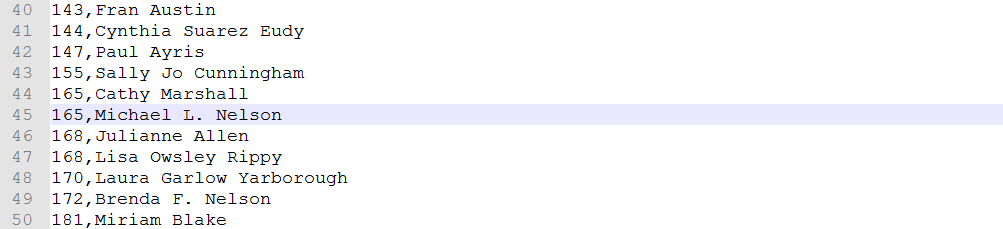
\includegraphics[width=6.5in]{sortedfacefriend.png}
\caption{Sample of part of sortedfacefriend.txt}
\end{figure}

Next, I load this sorted file into R and plotted the graph. The mean, median, and standard deviation are also calculated in R.

\lstinputlisting[language=R]{FaceFriendCounts.R}

\begin{figure}[h]
\centering
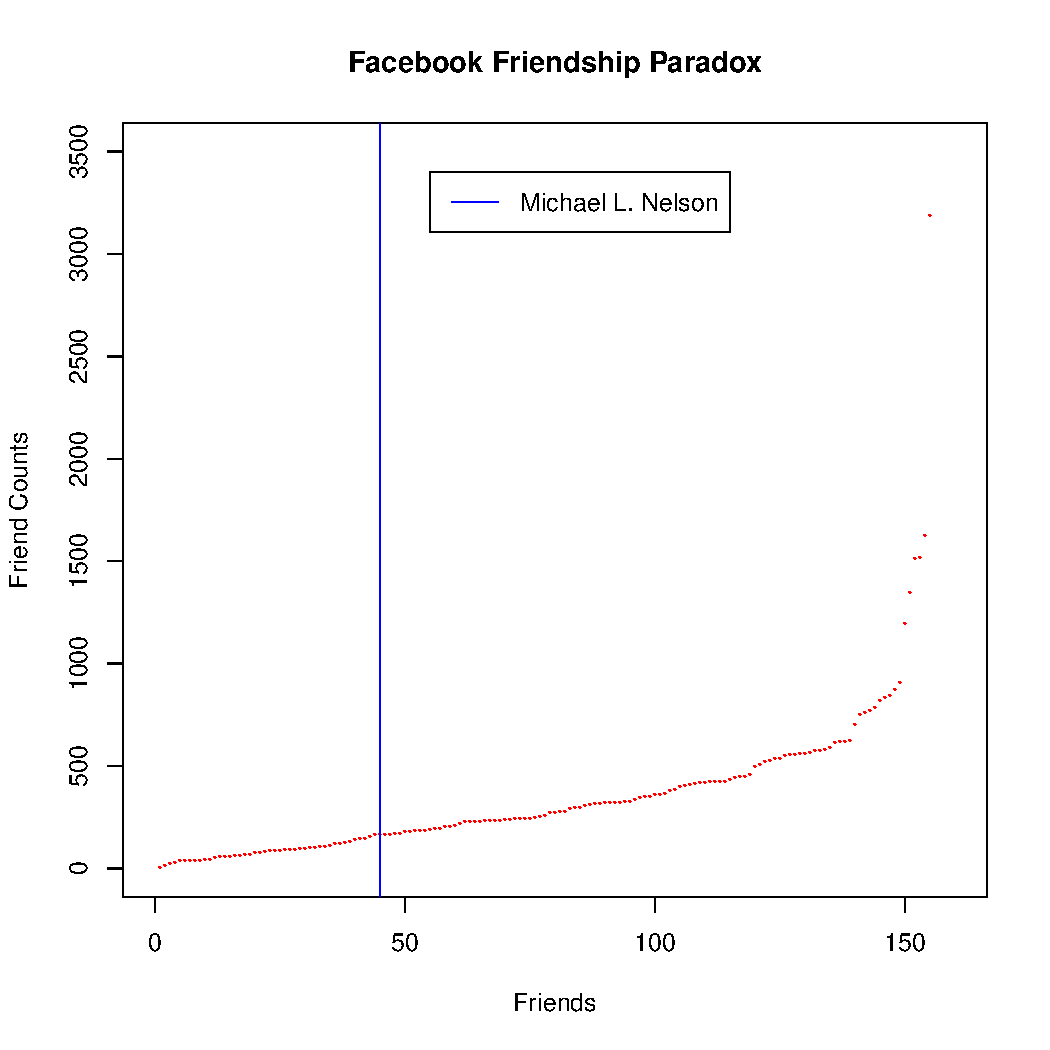
\includegraphics[width=5in]{FaceFriends.pdf}
\caption{A dot graph of friend counts per friend}
\end{figure}

\noindent
Dr. Nelson's Friends: 165

\noindent
Mean: 357.74

\noindent
Median: 259

\noindent
Standard Deviation: 370.7

There are 11 individuals who do not have the ``friend\_count" attribute in their nodes. Therefore, they are not included in the graph and calculations.

The Friendship Paradox holds true for Dr. Nelson's Facebook account. Looking at the graph, we can see that he is located at the left side of the graph, which means that most of his friends have more friends than him on Facebook.

\section*{Problem 2}
Determine if the friendship paradox holds for your Twitter account.
Since Twitter is a directed graph, use ``followers" as value you measure
(i.e., ``do your followers have more followers than you?").

Generate the same graph as in question \#1, and calcuate the same 
mean, standard deviation, and median values.

\noindent
For the Twitter 1.1 API to help gather this data, see:

\noindent
\begin{verbatim}
https://dev.twitter.com/docs/api/1.1/get/followers/list
\end{verbatim}

If you do not have followers on Twitter (or don't have more than 50),
then use my twitter account ``phonedude\_mln".



\subsection*{Answer}

To solve this problem, I revisited a program from assignment 2 and made some changes. This time, instead of stream listen for links in people's tweets, we are looking for the followers count of ``phonedude\_mln" and its followers. I decide to use tweepy this time, because it seems to be simpler and more suited to handle this problem. First, gain access with my consumer and access keys and tokens. Then, I get the follower count of ``phonedude\_mln" and write it to a file along with the screen name, which is ``phonedude\_mln". Next, I get phonedude\_mln's followers and the follower count for each of them. I did encounter an issue at this part. To protect its server from overwhelming traffics, Twitter has set limitations on access rate. Since I used tweepy's cursor function, I am limited to 15 calls in a period of 15 minutes. However, with 15 calls, I was only able to get 300 follower counts before being kicked out by Twitter(phonedude\_mln had 489 followers at that time, the number has increased to 491 the next day). I did try to solve this issue by setting a sleeping period of 60s*15, but it gives me issues as well. At the end, I solved this problem by increasing the size of each call page. Tweepy cursor has a default setting of 20 items per call page, therefore, all I had to do is to increase the items per page. Just because I can, I set the page size to its maximum, which is 200, and I was able to get all of the follower screen names and their follower counts in 3 calls. 

\lstinputlisting[language=python]{twitterFriends.py}

\noindent
Again, I sorted the list by by using sort -n and saved to a file called sortedCount.txt.
\pagebreak

\begin{figure}[h]
\centering
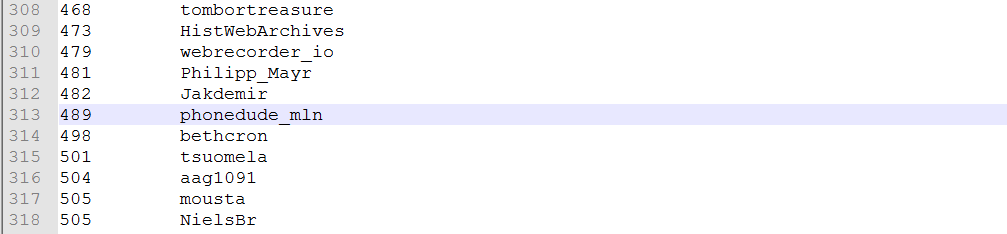
\includegraphics[width=6.5in]{tSordedCount.png}
\caption{Sample of part of sortedCount.txt}
\end{figure}

\noindent
With this sorted file, I loaded the data into R and plotted the graph. Below are the R code and graphs. 

\lstinputlisting[language=R]{twitterGraph.R}

\newpage

\begin{figure}[h]
\centering
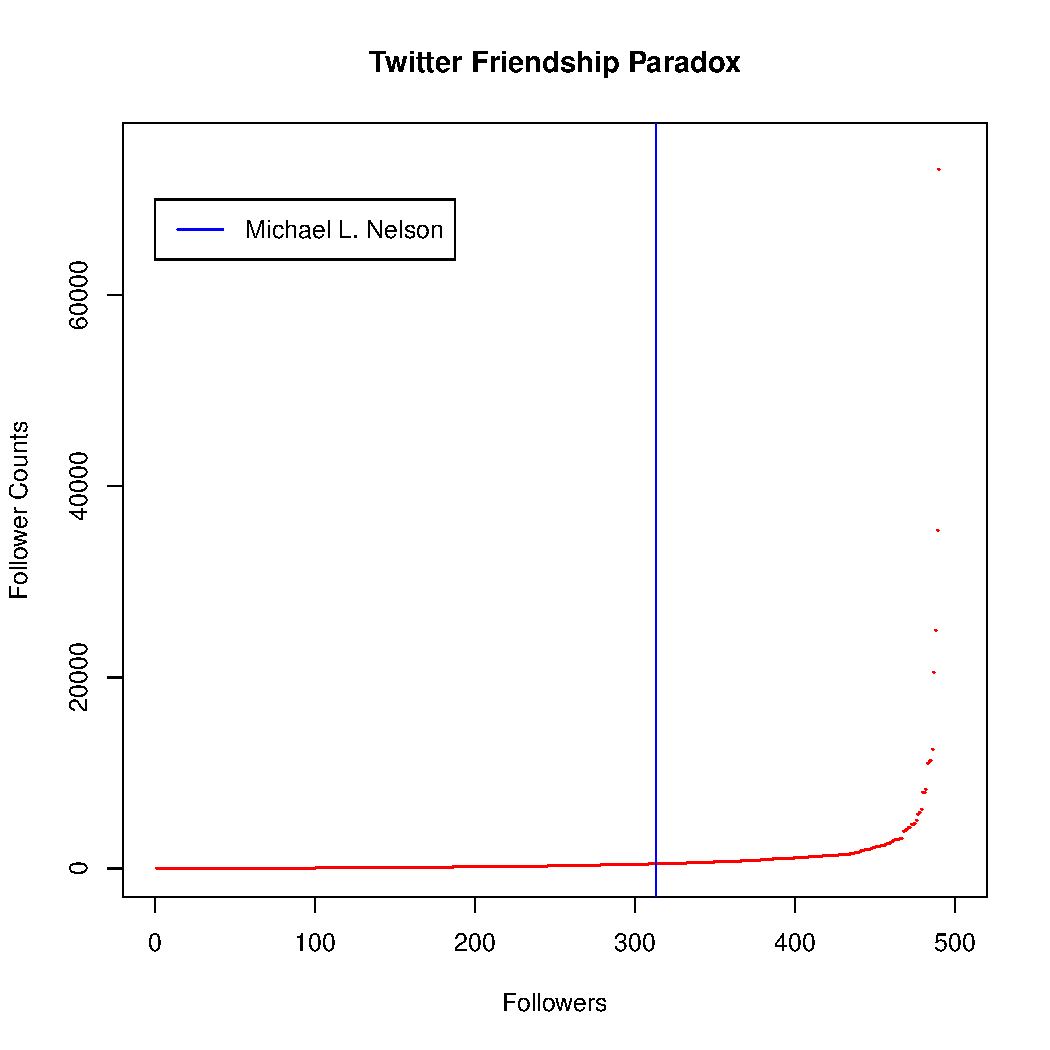
\includegraphics[width=5in]{TwitterFollowers.pdf}
\caption{A dot graph of follower counts per follower}
\end{figure}



Because of few individuals who have many more followers than other users, it made this graph hard to read. To make this graph more comprehensive, I changed the y axis to log scale. However, logarithm does not work with 0, therefore, the six individuals who have 0 follower are not included in this graph.

\begin{figure}[h]
\centering
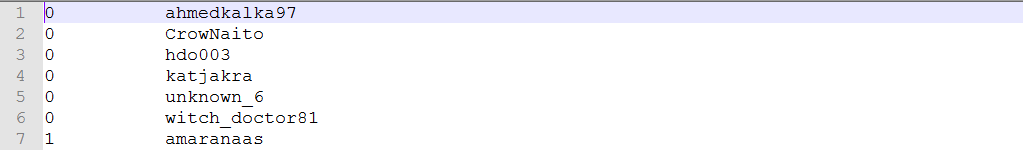
\includegraphics[width=6.5in]{twitterexcluded.png}
\end{figure}
\newpage

\begin{figure}[h]
\centering
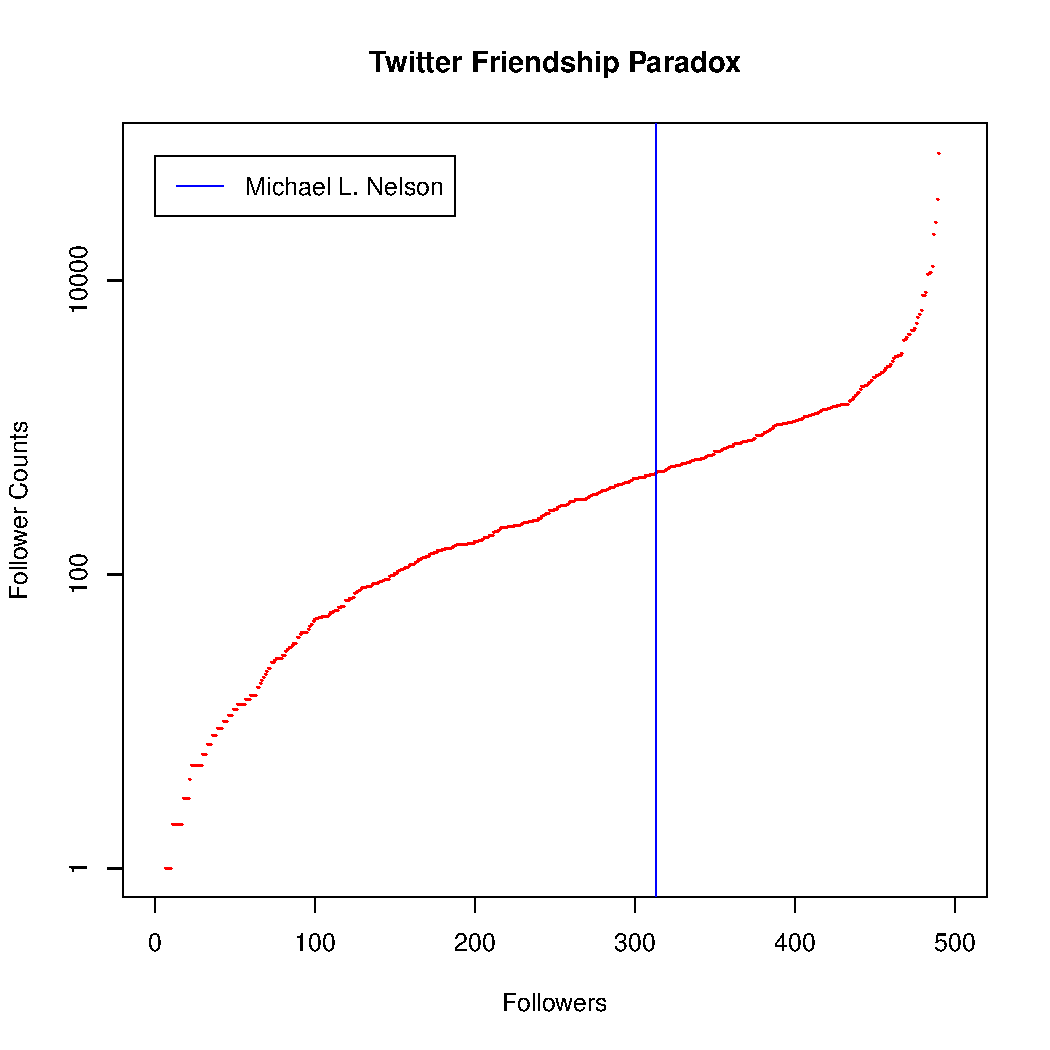
\includegraphics[width=5in]{TwitterFollowerslg.pdf}
\caption{Second dot graph of follower counts per follower}
\end{figure}

\noindent
Dr. Nelson's Followers: 489

\noindent
Mean: 1045.867

\noindent
Median: 259

\noindent
Standard Deviation: 4146.195

Interesting enough, the median for Dr. Nelson's followers' follower counts is also 259. I thought that I made a mistake at first, but after checking several times, I am certain it is 259. However, the number has change now since Dr. Nelson has gained few more followers. 

The Friendship Paradox does not hold true for Dr. Nelson's Twitter account. Based off the graph, we can see that Dr. Nelson is located towards the right side of the graph, which means that most of Dr. Nelson's followers have less followers than Dr. Nelson.



\end{document}